\section{实现与实验}

\begin{figure}[t]
    \centering
    \begin{subfigure}[b]{\linewidth}
        \centering
        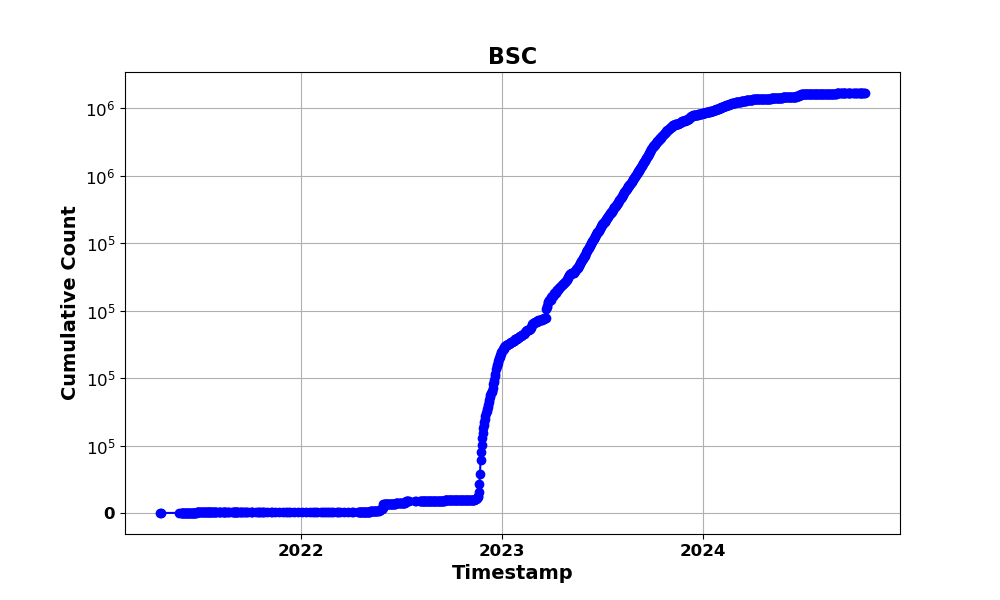
\includegraphics[width=\linewidth]{Sections/Picture/BSC.png}
        \caption{BSC}
        \label{fig:bsc}
    \end{subfigure}
    \vfill
    \begin{subfigure}[b]{\linewidth}
        \centering
        
\includegraphics[width=\linewidth]{Sections/Picture/ETH.png}
        \caption{ETH}
        \label{fig:eth}
    \end{subfigure}
    \vfill
    \begin{subfigure}[b]{\linewidth}
        \centering
        
\includegraphics[width=\linewidth]{Sections/Picture/Polygon.png}
        \caption{Polygon}
        \label{fig:polygon}
    \end{subfigure}
    \caption{针对 9 个地址在不同平台上的 ERC-20 转账幻影事件分析。}
    \label{fig:phantom_events_across_platforms}
\end{figure}

\label{sec:evaluation}
我们的工具采用 Python 实现，支持对智能合约进行字节码级和源代码级分析，同时支持交易级监控。对于字节码级分析，我们使用 Gigahorse 框架从已编译字节码中构建 ICFG。在源代码级，我们的工具支持所有与 Slither~\cite{Slither} 兼容的 Solidity 版本，使我们能够提取 AST，并对事件发出和参数约束进行详细分析。我们采用 Z3~\cite{Z3} 作为约束求解器，用于处理符号执行并消除不可行路径。此外，该工具还包含一个交易级链下监控系统，能够解析链上数据，并应用自定义规则检测异常和验证攻击交易是否成功。所有主要组件，包括字节码分析引擎、源代码符号执行器和交易监控系统，均由我们开发。该实现基于 Python，代码量超过 5,000 行。


\begin{itemize}%[leftmargin=*,topsep=2pt]
  \item \textbf{RQ1} \textit{幻影事件在主流区块链平台上有多普遍，\tool 在交易级检测中的表现如何？} 我们旨在理解验证者通过合约地址和源函数验证事件来源的必要性。
  \item \textbf{RQ2} \textit{\tool 从智能合约中检测潜在幻影事件的效果如何？} 我们开发了 \tool，并构建了一个自定义基准来评估其有效性。
  \item \textbf{RQ3} \textit{在真实世界中实施此类攻击的可行性如何？} 我们旨在验证所识别漏洞是否能够在真实场景中被实施。
\end{itemize}

\subsection{幻影事件的普遍性（RQ1）}

TokenScope~\cite{TokenScope} 等工具有助于检测代币行为中的不一致性，Guoyi Ye 等人~\cite{wallet_visual}也展示了转账事件中伪造用户地址的普遍性。我们旨在探索两个具体方面：幻影事件攻击中可疑地址的普遍性，以及此类攻击是否在跨链桥中常见。

\subsubsection{方法}

为更好地理解幻影事件在真实世界中的发生情况，我们使用区块链交易数据进行了两个独立实验。

在第一个实验中，我们重点关注九个特定伪造地址，即从 \emph{0x1111...1111} 到 \emph{0x9999...9999}，因为这些地址在正常交易中被生成或使用的可能性极低。我们检查了截至 2024 年 10 月 21 日在 Ethereum、BSC 和 Polygon 区块链上的交易，寻找源自这些地址的 ERC-20 代币转移。该方法有助于衡量不同区块链平台上幻影事件的普遍性。

在第二个实验中，考虑到跨链桥高度易受幻影事件攻击影响，我们基于交易级分析为跨链桥创建了检测规则。我们使用 XScope~\cite{Xscope} 的相关数据集，将结果与其发现进行比较；XScope 是目前唯一已有的桥攻击交易检测工具。


\subsubsection{结果}

%\begin{table}[t]
%\caption{Analysis of ERC-20 transfer phantom events across different platforms for 9 addresses.}
%\centering
%\begin{tabular}{ll}
%\toprule
%\textbf{Platforms} & \textbf{Potential Phantom Events} \\
%\midrule
%Ethereum & 18,099 \\
%BSC & 1,243,917 \\
%Polygon & 436,477 \\
%\midrule
%\textbf{Total} & \textbf{1,661,813} \\
%\bottomrule
%\end{tabular}
%\label{table:phantom_events_across_platforms}
%\end{table}



在第一个实验中，我们围绕九个特定地址进行分析，识别出 ERC-20 代币转账中存在大量幻影事件，如\cref{fig:phantom_events_across_platforms}所示。我们在 Ethereum 上发现 18,099 个此类事件，在 BSC 上发现 1,245,125 个，在 Polygon 上发现 436,407 个。如果这些事件未被适当验证，可能导致安全漏洞利用。仅九个地址就出现如此显著的事件数量，凸显了严格交易验证对于维护区块链操作安全性和可信度的关键必要性。


%\begin{table}[htbp]
%    \centering
%    \caption{Number of detected attack transactions by tools.}
%    \label{tab:attack_detection}
%    \begin{tabular}{lrr}
%        \toprule
%        \textbf{Project} & \textbf{XScope} & \textbf{\tool} \\
%        \midrule
%        THORChain \# 1 & 9 & 9 \\
%        THORChain \# 2 & 41 & 48 \\
%        pNetwork & 3 & 5 \\
%        Qubit Bridge & 20 & 20 \\
%        meter.io & N/A & 5 \\
%        CENNZnet & N/A & 1 \\
%        \bottomrule
%    \end{tabular}
%\end{table}

\begin{table}[t]
    \centering
    \caption{不同工具检测到的攻击交易数量和成功攻击数量。}
    \label{tab:attack_detection}
    \begin{tabular}{l r r r}
        \toprule
        \textbf{项目} & \textbf{XScope} & \multicolumn{2}{c}{\textbf{\tool}} \\
        \cmidrule(lr){2-2} \cmidrule(lr){3-4}
        & \textbf{攻击} & \textbf{攻击交易} & \textbf{成功攻击} \\
        \midrule
        THORChain \#1 & 9 & 9 & 9 \\
        THORChain \#2 & 41 & 48 & 41 \\
        pNetwork & 3 & 5 & 3 \\
        Qubit Bridge & 20 & 20 & 20 \\
        meter.io & N/A & 5 & 5 \\
        CENNZnet & N/A & 1 & 1 \\
        \bottomrule
    \end{tabular}
\end{table}


在第二个实验中（结果如\cref{tab:attack_detection}所示），我们检测到了 XScope 报告的所有交易，并识别出了额外的攻击交易。XScope 只记录攻击已经发生的交易，其标志是目标链上发生了资金转移。相比之下，我们能够在转账发生前检测攻击，从而帮助项目团队主动识别攻击者。我们还检测到了 meter.io~\cite{Meter} 上的攻击交易；XScope 虽然在其攻击事件列表中提到了该项目，但并未进行分析。此外，我们在 CENNZnet 上发现了一笔攻击交易，造成了 150 ETH 的损失。该事件此前未被任何其他工具或安全公司披露或报告。

\vspace{\baselineskip}
\begin{mdframed}
\noindent\textbf{对 RQ1 的回答：} \textit{我们的分析表明，仅基于九个地址，就能发现 Ethereum、BSC 和 Polygon 上存在大量幻影事件。此外，与当前先进工具相比，我们的检测规则展现出了有效性。}
\end{mdframed}

\subsection{从代码中检测幻影事件（RQ2）}

\subsubsection{数据集}
SmartAxe~\cite{liao2024smartaxe} 和 XGuard~\cite{wang2024xguard} 是目前已知的两个用于检测跨链漏洞的工具，其中 SmartAxe 侧重于字节码级分析，而 XGuard 提供源代码级分析。

在对 SmartAxe 数据集的分析中，我们发现 20 起攻击中只有 8 起由\emph{事件仿冒}导致，并且桥合约中存在存在漏洞的函数路径对。我们重新标注了这 8 起攻击，并从 SmartAxe 分析的 129 个桥中额外添加了 29 对受\emph{事件仿冒}影响的函数路径。作为补充，我们从 BSC~\cite{bscdata} 中 452,666 个已验证合约中，使用 TF-IDF 算法选择了 500 个相似度较低的 BSC 智能合约并进行人工标注。去重后，我们额外识别出 80 对受\emph{事件仿冒}影响的函数对。

通过结合 SmartAxe 和 XGuard 数据集以及人工标注的函数对，我们构建了一个综合数据集，其中包含 117 对受\emph{事件仿冒}影响的函数对，用于评估我们的检测工具。

为检测\emph{不一致日志记录}，我们使用了一个由 28 个经人工审计的不一致日志记录参数案例组成的数据集，这些案例是在我们的审计过程中识别出来的。

\subsubsection{结果}

\begin{table*}[htbp]
    \centering
    \caption{事件仿冒与不一致日志记录检测中的工具比较}
    \label{tab:tool_result}
    \small
    \begin{tabular}{p{3.9cm}ccc ccc}
        \toprule
        \multirow{2}{*}{\textbf{工具}} & \multicolumn{3}{c}{\textbf{事件仿冒}} & \multicolumn{3}{c}{\textbf{不一致日志记录}} \\
        \cmidrule(lr){2-4} \cmidrule(lr){5-7}
        & \textbf{精确率} & \textbf{召回率} & \textbf{F1} & \textbf{精确率} & \textbf{召回率} & \textbf{F1} \\
        \midrule
        SmartAxe & 40.50\% & 25.12\% & 31.01\% & N/A & N/A & N/A \\
        XGuard & 87.75\% & 55.12\% & 67.70\% & 64.71\% & 91.75\% & 75.82\% \\
        \tool (Bytecode) & 84.0\% & 100\% & 91.30\% & 62.50\% & 16.12\% & 39.31\% \\
        \tool (Source) & 90.83\% & 86.51\% & 88.62\% & 90.30\% & 100\% & 94.90\% \\
        \bottomrule
    \end{tabular}
\end{table*}
在实验中，如\cref{tab:tool_result}所示，\tool 在检测\emph{事件仿冒}和\emph{不一致日志记录}漏洞方面均显著优于 SmartAxe 和 XGuard。对于\emph{事件仿冒}，SmartAxe 的 F1 分数为 31.01\%，精确率为 40.50\%，召回率为 25.12\%；XGuard 的 F1 分数为 67.70\%，精确率为 87.75\%，召回率为 55.12\%。相比之下，\tool 表现更优，在字节码级达到 91.30\% 的 F1 分数，在源代码级达到 88.62\% 的 F1 分数。对于\emph{不一致日志记录}检测，\tool 同样优于 XGuard，在召回率达到 100\% 的情况下取得了 94.9\% 的 F1 分数，而 XGuard 的 F1 分数为 75.82\%。

\tool 的字节码级实现和源代码级实现之间的性能指标差异，凸显了两种方法各自的局限性。在\emph{事件仿冒}检测中，\tool 的字节码级分析缺乏约束验证，因此可能将缺少充分伪造证据的事件标记出来，导致精确率较低。然而，在源代码级，\tool 会执行全面的约束检查，从而显著提高精确率。对于\emph{不一致日志记录}，\tool 的字节码分析仅限于索引参数，因此无法识别与非索引参数相关的问题，进而降低召回率。在具备源代码访问权限时，\tool 可以同时分析索引参数和非索引参数，因此取得更高召回率。相比之下，SmartAxe 和 XGuard 存在固有设计限制：SmartAxe 只检测两个函数是否发出同一事件，而不考虑调用路径中的约束验证；XGuard 则关注单个函数内部的约束，缺乏函数间分析。通过同时分析函数交互和调用路径，\tool 能够检测其他工具遗漏的漏洞，并在\emph{事件仿冒}和\emph{不一致日志记录}检测中取得更优结果。


\subsubsection{局限性}

评估中的误报和漏报揭示了本文方法的两个主要局限。首先，在处理不完整合约代码时，例如某些函数中的接口调用，我们计算得到的约束未必总是精确，这会导致约束较弱并进而产生误报。其次，由于 Solidity 编译缺陷，一些已通过区块链浏览器验证的智能合约在使用我们的工具进行分析时出现编译错误~\cite{compile_issue}。解决这些局限将是我们未来工作的重点。


\vspace{\baselineskip}
\begin{mdframed}
\noindent\textbf{对 RQ2 的回答：} \textit{\tool 在检测幻影事件漏洞方面被证明高度有效，并在精确率、召回率和 F1 分数上超过了当前先进工具。}
\end{mdframed}

\subsection{真实世界攻击可行性（RQ3）}
\subsubsection{方法}
我们将工具应用于多个区块链平台进行测试，旨在识别智能合约中与幻影事件攻击相关的漏洞。除链上测试外，我们还审计了多种链下应用，包括区块链浏览器、NFT 市场和加密货币钱包。这些审计侧重于评估安全协议，并识别可能被幻影事件利用的潜在漏洞，从而确保对链上和链下组件进行全面分析。

所有已识别的幻影事件漏洞均在受控本地环境中通过模拟场景进行测试，以确保不会对真实世界区块链平台造成干扰或损害。

\subsubsection{结果}

在实验中，我们识别出一笔\emph{转账事件欺骗}交易，其中一次虚假转账看起来像是将代币从地址 \textit{0x8888...8888} 转入受害者钱包。尽管实际上并未发生任何代币转账，至少五个主要区块链浏览器 BscScan、OKLink、Bitquery、Tokenview 和 Bsctrace~\cite{bscscan,oklink,bitquery,tokenview,bsctrace} 都错误地将该欺骗事件识别为合法交易。这凸显了链下系统中的普遍脆弱性，即它们难以区分真实事件和幻影事件。

此外，我们在两个领先 NFT 市场 Opensea 和 Rarible 的测试网环境中成功复现了 ``sleepminting'' 攻击。尽管已有用于检测此类攻击的监控方案，但完全缓解这些漏洞仍是一项持续挑战。

此外，在安全审计过程中，我们在六个加密货币钱包中发现了关键漏洞，并将其报告给相应项目团队或通过漏洞赏金平台报告。其中四个漏洞已被确认，一个漏洞为我们带来了来自项目团队的 600 美元赏金。

在对多个区块链桥的审计中，我们识别出链下代码中的漏洞，使这些桥暴露于仿冒合约攻击之下。在该攻击中，恶意合约会发出伪造事件，而链下系统会错误地将其作为合法事件处理。我们发现的一个存在漏洞的系统曾被某个公链项目分叉并部署，截至 2024 年 10 月 9 日，该项目市值超过 2.5 亿美元。这些漏洞已报告给相应项目团队以便修复。


此外，我们在流行区块链浏览器 Blockscout~\cite{error_display} 中识别出一个事件数据显示问题，该问题可能损害交易记录的准确性。该缺陷可能导致用户误解区块链数据，从而削弱其对交易历史的信任。

在对多个活跃智能合约项目的审计中，我们还发现三个 DeFi 项目和一个 GameFi 项目易受\emph{不一致日志记录}攻击影响，该漏洞由本文首次提出（见\ref{vec:attack2}）。在这组项目中，受影响项目的最高市值为 169,688 美元。


\vspace{\baselineskip}
\begin{mdframed}
\noindent\textbf{对 RQ3 的回答：} \textit{我们的研究表明，幻影事件攻击在真实世界区块链平台上具有可行性，具体目标包括区块链浏览器、NFT 市场、DeFi、GameFi 和加密货币钱包。这强调了在区块链生态系统中改进安全措施的迫切需求。详细报告和确认案例可见补充材料。}
\end{mdframed}


\subsection{有效性威胁}
内部有效性威胁主要源于人工数据标注过程中可能引入的不准确性。为提高数据标注准确性，我们采用了三层方法：两名作者独立标注数据，第三名作者审查其标注结果。该方法在三个不同层级进行了彻底审查，以提高数据集分类的精确性。

为确保外部有效性，我们使实验中使用的数据集类型和来源更加多样化。除 SmartAxe 和 XGuard 提供的以桥为中心的数据外，我们还扩展了数据集，使其包含更广泛的场景。此外，我们避免使用相似度较高的智能合约，以提高分析的多样性和有效性。
